
\begin{table}[htbp]
\centering
\caption{Überblick über die Hyperparameter des DDPG-Modells inklusive Parameterraum}
\label{tab:hyperparameters_Phase2}
\begin{tabular}{lc}
\hline
\textbf{Parameter} & \textbf{Wert} \\
\hline
ALPHA & \( 1 \times 10^{-6} \) \\
WORKER & 6 \\
ITERATION & 1 \\
STEPS & 60000 \\
BATCH\_SIZE & 500 \\
EXPLOITATION & 10 \\
LAYERS & 24 \\
LAYER\_1 & 158 \\
LAYER\_2 & 52 \\
NOISE & 0.45 \\
GAMMA & 0.0 \\
MAX\_KP & 1000.0 \\
MAX\_KI & 100.0 \\
MAX\_KD & 10.0 \\
\hline
\end{tabular}
\end{table}

In dieser Phase unserer Untersuchung konzentrieren wir uns auf die vertiefte Analyse des Lernprozesses unter Berücksichtigung der modifizierten Belohnungsfunktion und der Erweiterung des Suchraums. Diese Phase ermöglicht es uns, ein detailliertes Verständnis dafür zu entwickeln, wie unsere Modelle auf diese Änderungen reagieren und sich anpassen.

\paragraph{Anpassung der Belohnungsfunktion}
Um eine differenziertere Reaktion auf Spannungsabweichungen zu erzielen, haben wir die Belohnungsfunktion angepasst. Für größere Abweichungen, spezifisch über einem Schwellenwert von 1, wird eine quadratische Bestrafung angewendet, um auf diese stärker zu reagieren. Dies verbessert die Stabilität des Systems bei größeren Spannungsschwankungen. Für kleinere Abweichungen, die unter diesem Schwellenwert liegen, wird eine Bestrafung auf Basis des absoluten Wertes vorgenommen. Dies macht das System sensibler für kleinere Spannungsabweichungen und ermöglicht eine feinere Justierung.

\paragraph{Erweiterung des Suchraums}
Wir haben den Suchraum erheblich erweitert, um eine größere Bandbreite an Konfigurationsmöglichkeiten zu erforschen. Dies erlaubt es uns, die Robustheit unserer Modelle in einem größeren und komplexeren Parameterraum zu testen. Insbesondere wollten wir untersuchen, wie die Bayesianische Optimierung, die in größeren Räumen typischerweise Herausforderungen begegnet, im Vergleich zum DDPG-Modell abschneidet. Diese Erweiterung hilft auch dabei, die Flexibilität und Anpassungsfähigkeit unserer Modelle in Szenarien mit weniger definierten Parametern zu demonstrieren.

\begin{figure}[htbp]
\centering
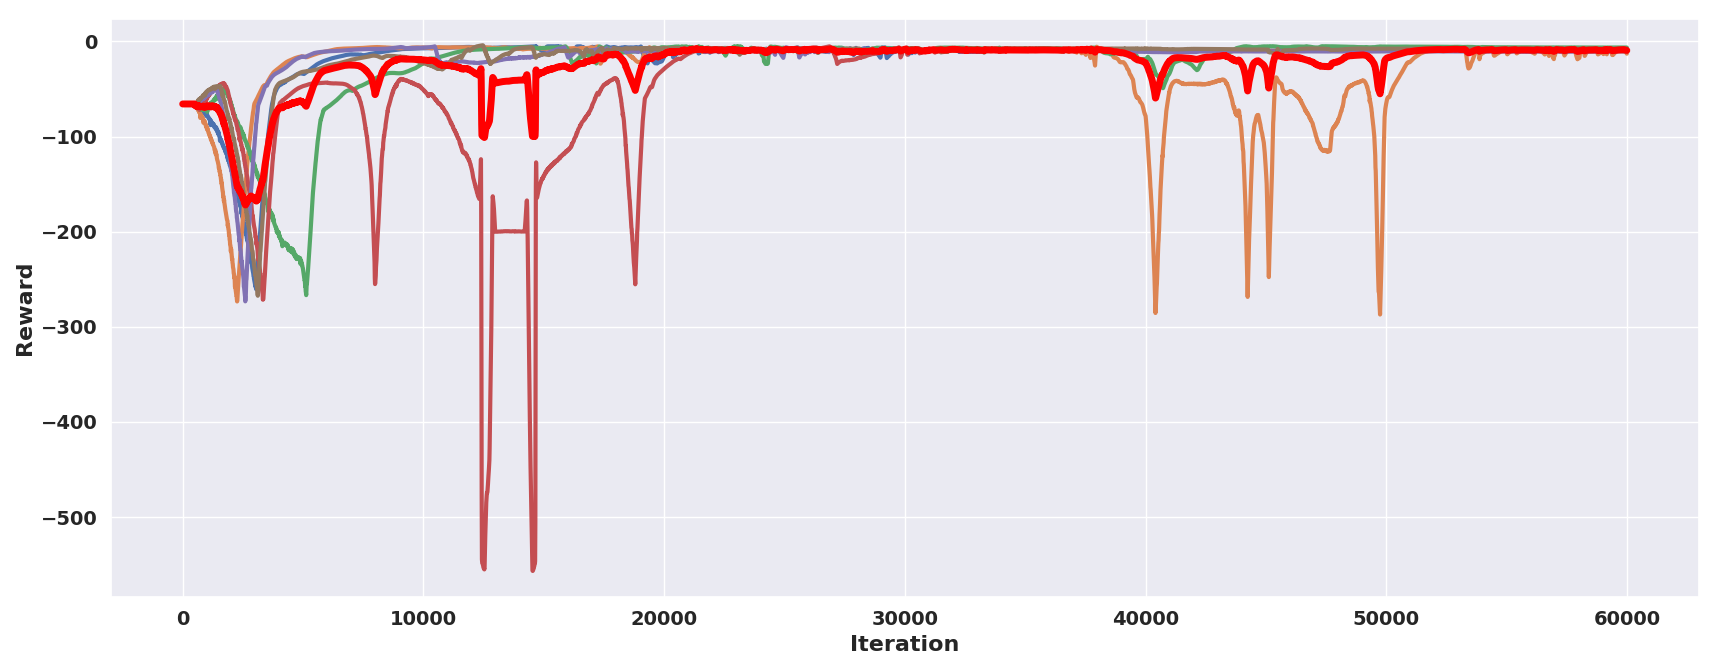
\includegraphics[width=\textwidth]{4Ergebnisse/Phasen/2Phase/2Phase.png}
\caption{Gesamtansicht des Lernprozesses des DDPG-Modells.}
\label{fig:phase 2 whole lern process}
\end{figure}

\paragraph{Detaillierte Darstellung des Lernprozesses}
Um die Entwicklung und Konvergenz unserer Modelle zu veranschaulichen, werden wir den Lernprozess detailliert darstellen, einschließlich visueller Darstellungen und Screenshots. Diese Darstellung soll den Fortschritt der Modelle im Laufe des Trainings verdeutlichen und zeigen, wie sie sich den neuen Herausforderungen stellen und anpassen. Durch die Kombination von modifizierter Belohnungsfunktion und erweitertem Suchraum können wir die Vielseitigkeit und Leistungsfähigkeit unserer Ansätze in einer breiten Palette von Anwendungsfällen aufzeigen. Während dieses Trainingsprozesses wurde eine beträchtliche Anzahl von Epochen genutzt. Die gewählte Lernrate war dabei bewusst gering gehalten, um eine stabile Konvergenz zu gewährleisten. Wie aus dem Graphen ersichtlich, haben die meisten Modelle eine signifikante und positive Konvergenz gezeigt, was auf die Effektivität des Lernansatzes und die ausgewählten Hyperparameter schließen lässt.


